\documentclass[10pt,mathserif]{beamer}
\usepackage{graphicx,amsmath,amssymb,tikz,psfrag}

\input defs.tex
\input slide_format.tex

%% begin presentation

\title{\large \bfseries Introduction to Python}

\author{Steven Diamond \and Jaehyun Park \\[1ex]
CS Department\\[1ex]
Stanford University}
\date{SIST, Shanghai, March 26-28 2016}

\begin{document}

\frame{
\thispagestyle{empty}
\titlepage
}

\begin{frame}{What is Python?}
a general programming language, popular for scientific computing

\BIT
\item top 5 most popular language
\item fully open source, \ie, free
\item many high-quality numerical packages (\eg, NumPy, SciPy)
\EIT
\end{frame}

\begin{frame}{Setting up Python}
\BIT
\item many possible choices
\item our suggestions:
\BIT
\item Python 2.7
\item Anaconda
% or Python(x,y)
\EIT
\item installing packages
\BIT
\item \texttt{conda install numpy}
\item \texttt{pip install cvxpy}
\EIT
\EIT
\end{frame}

\begin{frame}[fragile]{Jupyter notebooks}
\BIT
\item a Jupyter notebook is an interactive file run in your browser
\item launch from command line with \texttt{jupyter notebook}
\item notebooks in the launch folder are listed
\begin{center}
  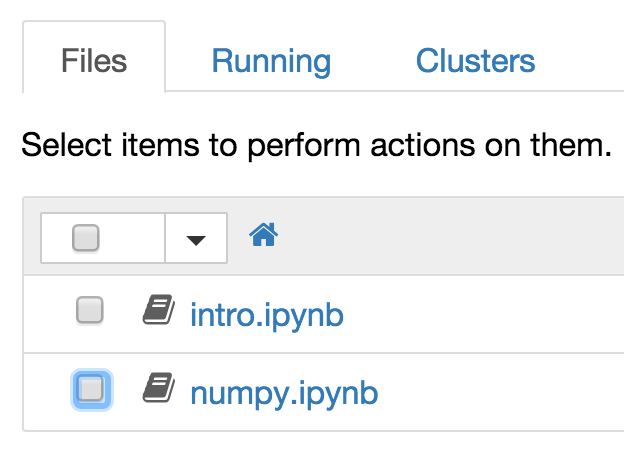
\includegraphics[height=0.20\textheight]{images/jupyter_load.png}
\end{center}
\item click on a notebook to open it
\item a new page should open in your browser that looks like
  \begin{center}
    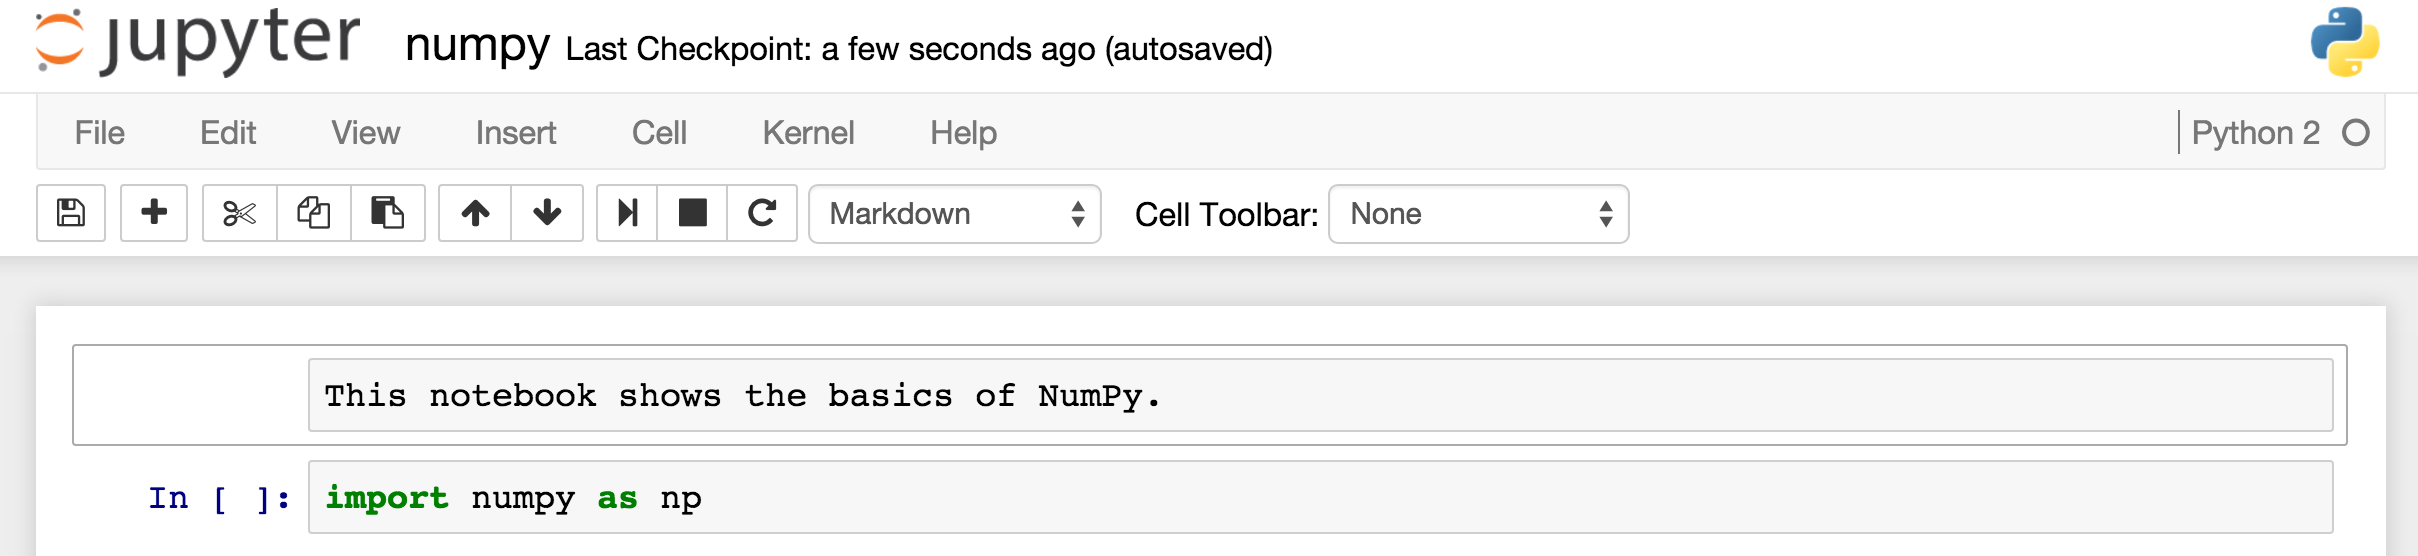
\includegraphics[height=0.15\textheight]{images/jupyter_example_notebook.png}
  \end{center}
\EIT
\end{frame}

% \item click on the \verb|New| button and select \texttt{Python 2}
%   \begin{center}
%     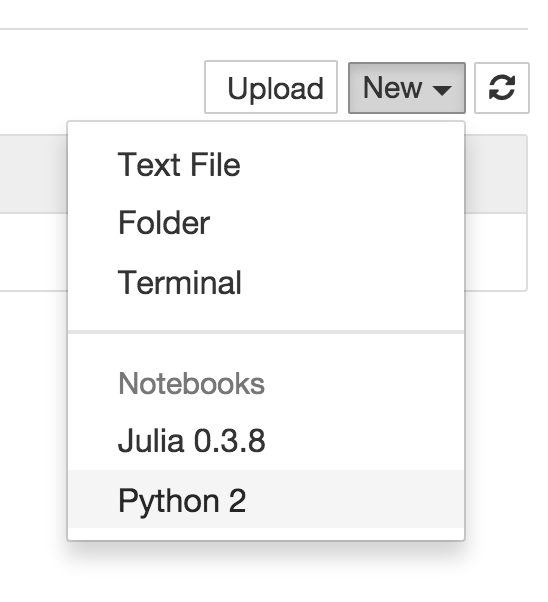
\includegraphics[height=0.20\textheight]{images/jupyter_new_button.png}
%   \end{center}
% \item a new page should open in your browser that looks like
%   \begin{center}
%     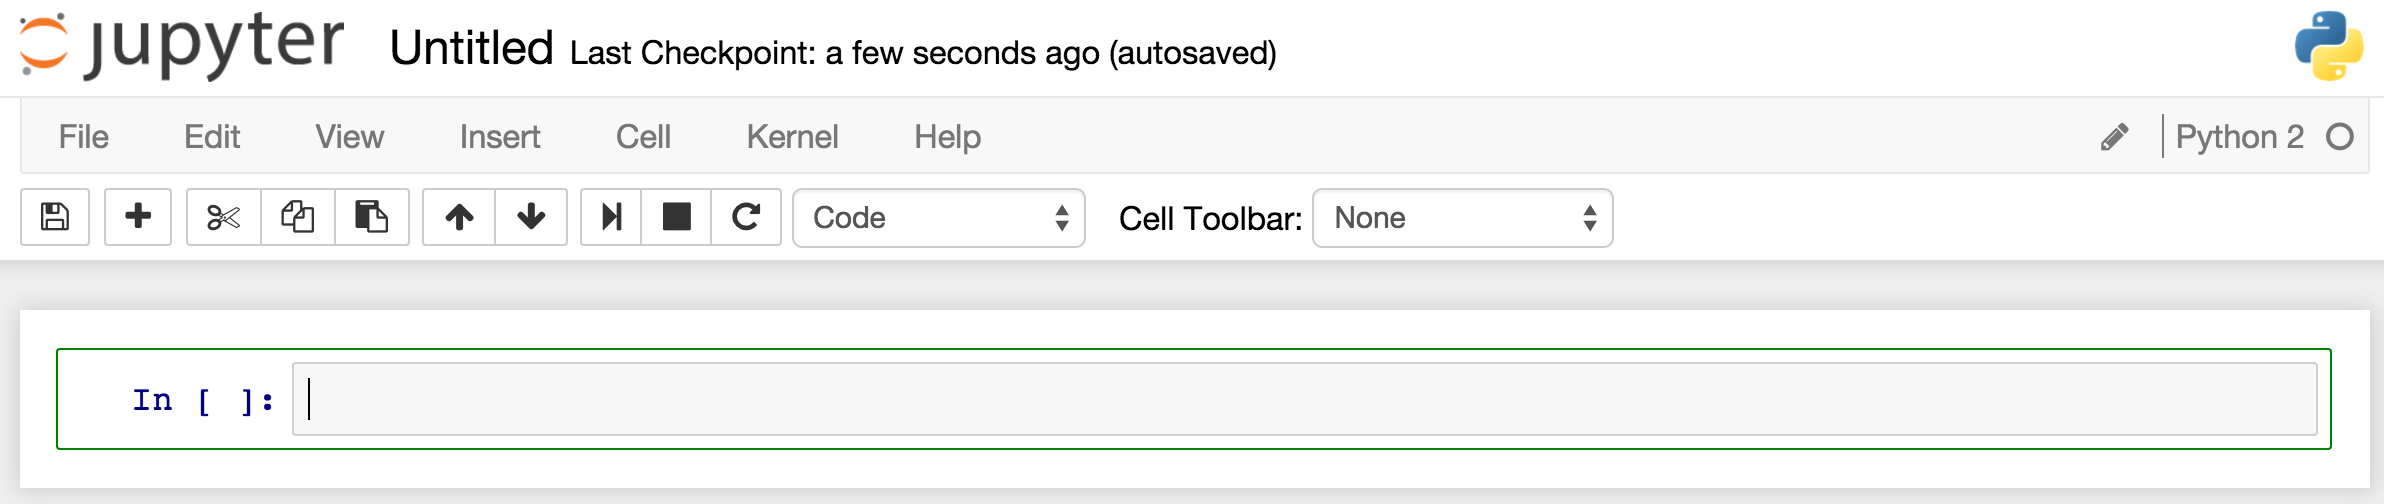
\includegraphics[height=0.15\textheight]{images/jupyter_notebook.png}
%   \end{center}
% \item you can rename you notebook by clicking on the name in the top left
%   \begin{center}
%     
\includegraphics[height=0.05\textheight]{images/jupyter_name.png}
%   \end{center}

\begin{frame}[fragile]{Coding in a Jupyter notebook}
\BIT
\item the Jupyter notebook is organized into cells
\item you can type code directly into a cell
  \begin{center}
    
\includegraphics[height=0.06\textheight]{images/jupyter_cell_input.png}
  \end{center}
\item you can run a cell by clicking it to select it, and then either clicking on the play button in the toolbar
  or pressing Shift + Enter
  \begin{center}
    
\includegraphics[height=0.05\textheight]{images/juliabox_play_button.png}
  \end{center}
\item the output of the cell will be displayed after it is run
  \begin{center}
    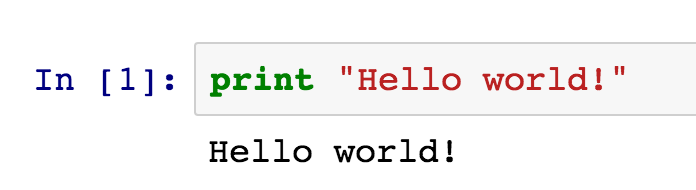
\includegraphics[height=0.1\textheight]{images/jupyter_cell_output.png}
  \end{center}
\item the menu bar will contain options for creating and deleting cells
  \begin{center}
    
\includegraphics[height=0.05\textheight]{images/juliabox_menu.png}
  \end{center}
\item make sure to periodically save your progress by clicking on the save button in the toolbar
  \begin{center}
    
\includegraphics[height=0.05\textheight]{images/juliabox_save_button.png}
  \end{center}
\EIT
\end{frame}

% \begin{frame}[fragile]{Including code in an IJulia notebook}
% \BIT
% \item you can include the code in the \verb|hello.jl| file you previously uploaded by creating and running a cell like
%   \begin{center}
%     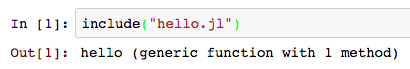
\includegraphics[height=0.10\textheight]{images/juliabox_include.png}
%   \end{center}
% \item once the code is included, you can run the \verb|hello| function that is included in \verb|hello.jl|
%   \begin{center}
%     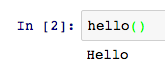
\includegraphics[height=0.10\textheight]{images/juliabox_hello.png}
%   \end{center}
% \EIT
% \end{frame}

% \begin{frame}[fragile]{Shutting down an IJulia notebook}
% \BIT
% \item to shut down an IJulia notebook, first close the IJulia notebook page in your browser
% \item return to your JuliaBox page, click on the notebook you wish to shut down, and then click the orange
% \verb|Shutdown| button
%   \begin{center}
%     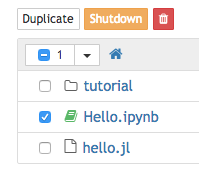
\includegraphics[height=0.25\textheight]{images/juliabox_shutdown.png}
%   \end{center}
% \EIT
% \end{frame}

\end{document}
